\chapter{Resultados y análisis}
\label{ch:resultados}

\begin{comment}
En este capítulo se exponen los diseños experimentales realizados para
comprobar el funcionamiento correcto del sistema. Por ejemplo, si se
realiza algún sistema con reconocimiento de patrones, usualmente esta
sección involucra las llamadas \emph{matrices de confusión} donde se
compactan las estadísticas de reconocimiento alcanzadas. En circuitos
de hardware, experimentos para determinar variaciones contra ruido,
etc. También pueden ilustrarse algunos resultados concretos como
ejemplo del funcionamiento de los algoritmos. Puede mostrar por medio
de experimentos ventajas, desventajas, desempeño de su algoritmo, o
comparaciones con otros algoritmos.

Recuerde que debe minimizar los ``saltos'' que el lector deba hacer en
su documento. Por tanto, usualmente el análisis se coloca junto a
\tablas y figuras presentadas, y debe tener un orden de tal modo que se
observe cómo los objetivos específicos y el objetivo general del
proyecto de tesis se han cumplido.



\section{Selección de modelos RL}

Como se mencionó en el capítulo \ref{ch:ControlPAMH}, los métodos de RL seleccionados para su implementación son el DQN y el PPO, por lo que se realizó la búsqueda de referencias 

\end{comment}

Este capítulo se presenta los resultados de la implementación de los modelos RL seleccionados para el control de la planta PAMH.

\section{Implementación de métodos RL}

Se ilustran a continación los experimentos realizados con los entornos virtuales de problemas clásicos de control, como el del péndulo invertido.

Luego se presentan los resultados de la implementación de los modelos DQN y PPO en el control de la planta simulada PAMH.

\subsection{Preparación del entorno virtual}

Para el caso del DQN la principal fuente fue \cite{PytorchDQN}, donde se detalla el funcionamiento de cada sección de los algoritmos de trabajo de DQN. 

El primer paso es montar el código base para el control del péndulo invertido con carrito (\textit{CartPole}), el cual solo requiere de la instalación de la paquetería necesaria para trabajar con tensores y procesamiento mediante CUDA.

El resultado de la primera prueba de implementación se ilustra en la figura \ref{fig:CartPole1}, donde el código base tiene como objetivo mantener el péndulo invertido apuntando hacia arriba el mayor tiempo posible. En este caso alcanzando las $500$ unidades del valor máximo de duración del episodio y demostrando la eficacia del DQN en el entrenamiento, en donde en aproximadamente el episodio $450$ de $600$, el agente aprende la táctica adecuada para mantener el equilibrio del péndulo.

%\begin{figure}[hh]
%	\centering
%	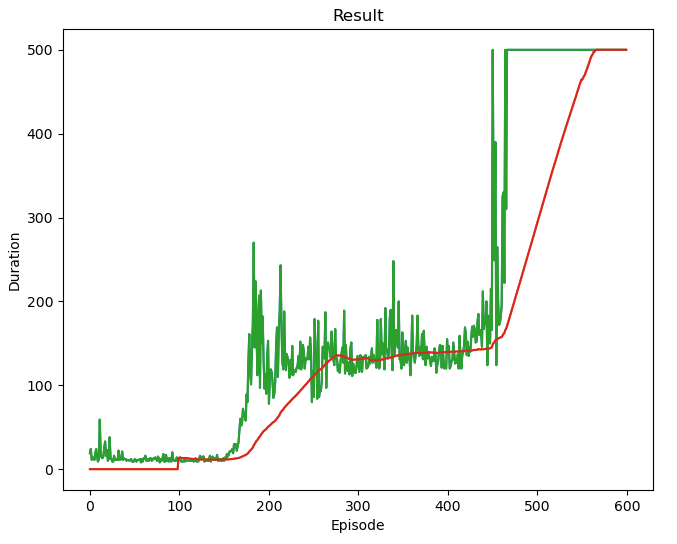
\includegraphics[scale=0.25]{fig/new/CartPole1.png}
%	\caption{}
%	\label{fig:CartPole1}
%\end{figure}



\begin{figure}[hh]
    \centering
    \begin{subfigure}[b]{0.45\textwidth}
        \centering
        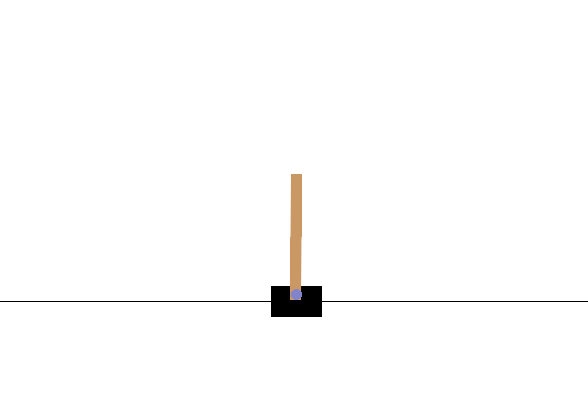
\includegraphics[width=\textwidth]{fig/new/CartPole1_1.png}
        \caption{ }
        \label{fig:figura1}
    \end{subfigure}
    \hfill
    \begin{subfigure}[b]{0.45\textwidth}
        \centering
        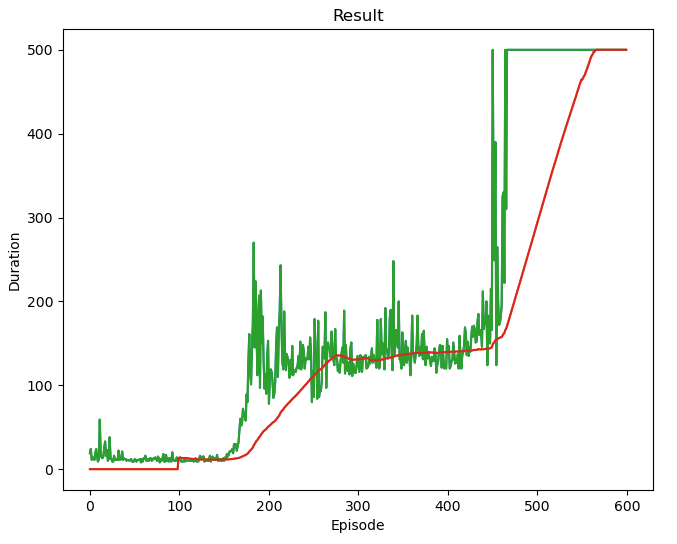
\includegraphics[width=\textwidth]{fig/new/CartPole1.png}
        \caption{ }
        \label{fig:figura2}
    \end{subfigure}
    \caption{Duración del episodio en prueba de implementación DQN con entorno \textit{CartPole}.}
    \label{fig:CartPole1}
\end{figure}


Como segundo paso se opta por el método PPO para trabajar con el péndulo invertido (\textit{Pendulum}), en este punto se definen las gráficas de recompensa, pérdida, tiempo de la iteración y duración del episodio, todos como valores promedio en el entrenamiento y se adiciona a la función de recompensa el factor de error angular $E_{\theta}$ de la ecuación (\ref{ecu:errorangular}), para indicar el $\theta_{objetivo}$. La prueba de implementación se muestra en la figura \ref{fig:Pendulum1} con el resultado de la prueba, donde se muestra un comportamiento inesperado por un ``atajo'' descubierto por el agente, obteniendo una recompensa promedio aceptable (curva azul) pero terminando el episodio prematuramente (curva morada), por lo que el castigo es menor, caso que debe ser ajustado o cubierto mediante la función de recompensas.



\begin{figure}[hh]
    \centering
    \begin{subfigure}[b]{0.3\textwidth}
        \centering
        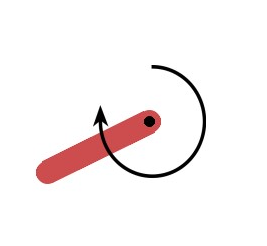
\includegraphics[width=\textwidth]{fig/new/Pendulum1_1.png}
        \caption{ }
        \label{fig:figura1_1}
    \end{subfigure}
    \hfill
    \begin{subfigure}[b]{0.6\textwidth}
        \centering
        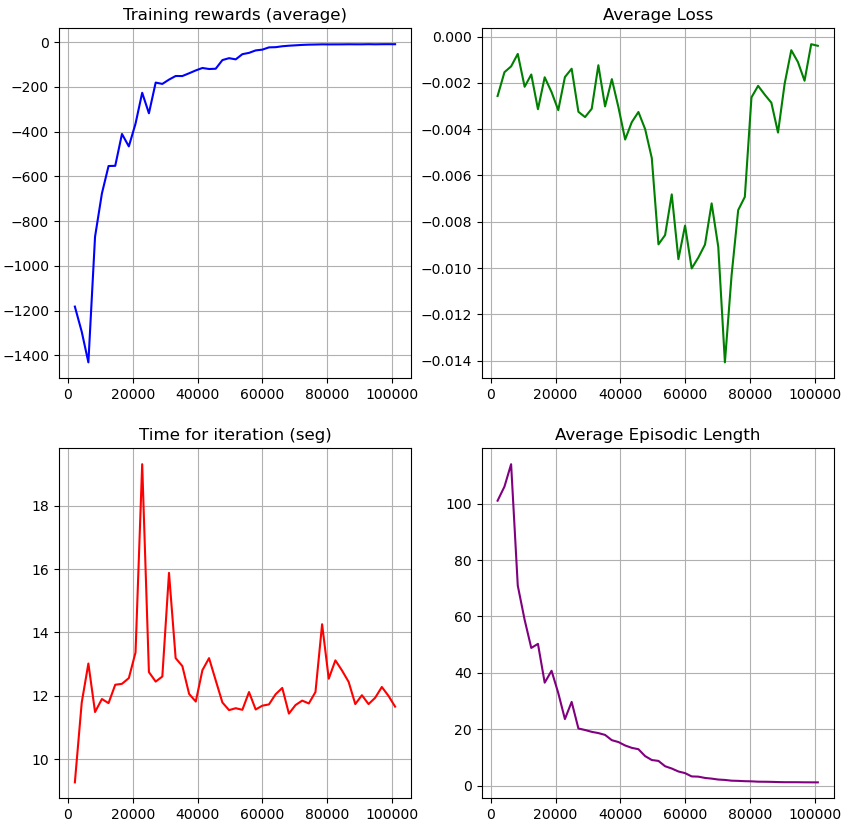
\includegraphics[width=\textwidth]{fig/new/Pendulum1.png}
        \caption{ }
        \label{fig:figura2_2}
    \end{subfigure}
    \caption{Proceso de entrenamiento con la implementación PPO con entorno \textit{Pendulum}.}
    \label{fig:Pendulum1}
\end{figure}


En este punto ya se cuenta con las bases necesarias del RL para la implementación de los métodos en el entorno virtual preparado con la RNAM del PAMH.

\subsection{Modelo DQN}

El código base del DQN tiene una implementación directa, pero el paso de discretización implicado en el enfoque mencionado a la RNAM del PAMH, aumenta el nivel del análisis y dificulta el proceso de entrenamiento. Una primera muestra de los resultados de los entrenamientos se ilustra en la figura \ref{fig:RewspromDQN}, donde se observa que la cualidad de discreto afecta a las recompensas obtenidas al generar saltos en las curvas, y una difícil aproximación al valor objetivo $\theta_{objetivo}=45^o$ lo cual es un reflejo directo de la baja recompensa que se recibe; sin embargo, se logra acercar al objetivo de manera prematura como se observa en la figura \ref{fig:AnglepromDQN}, indicando mejoría.

Al considerar la pérdida, se observa en la figura \ref{fig:LosspromDQN}, cómo los puntos de disminución de la pérdida coinciden con el aumento de recompensa, como el caso de los pasos (\textit{steps}) aproximados a $200$ y $900$, lo que se interpreta como un modelo que aprende y en el caso de DQN, logra predecir un correcto valor Q que aumenta la recompensa. Sin embargo, también es posible interpretar que las predicciones vuelven a perder el rumbo deseado, pues en puntos como el paso aproximado a $500$, la pérdida aumenta, indicando una pérdida de la predicción y por consiguiente, recompensa muy baja. Esto ocurre debido a que la componente exploratoria usada durante el entrenamiento desvía la atención del agente y lo lleva a condiciones donde no tiene experiencia para reaccionar adecuadamente.

%\begin{figure}[hh]
%	\centering
%	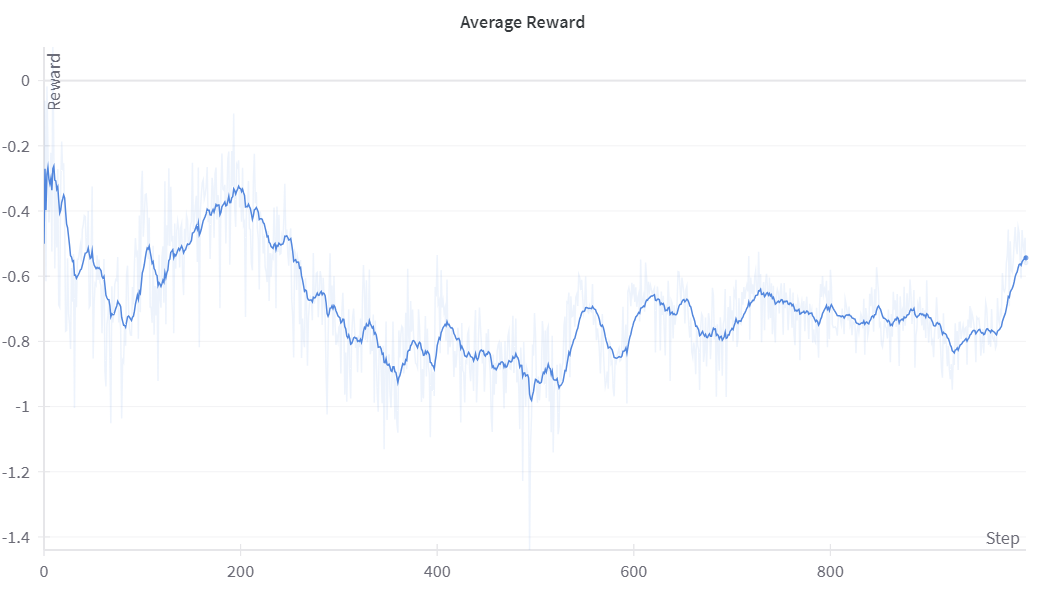
\includegraphics[scale=0.43]{fig/new/DQNentrenados.png}
%	\caption{Recompensa promedio de entrenamiento DQN.}
%	\label{fig:RewspromDQN}
%\end{figure}


\begin{figure}[hh]
    \centering
    \begin{subfigure}[b]{0.6\textwidth}
        \centering
        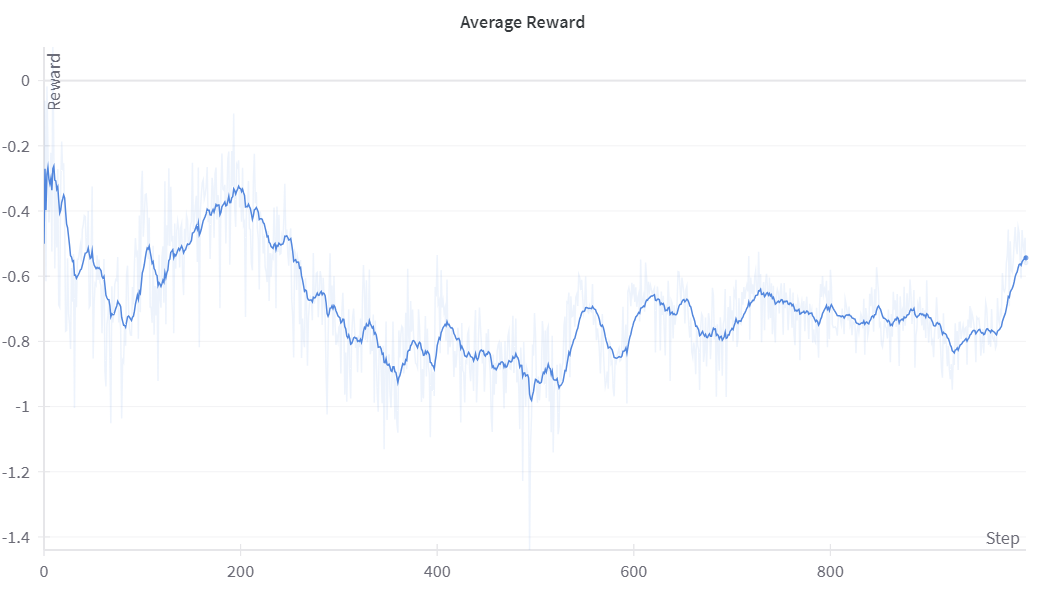
\includegraphics[width=\textwidth]{fig/new/DQNentrenados.png}
        \caption{Recompensa promedio del modelo DQN. La línea tenue en el fondo representa la señal completa, y la línea oscura dicha señal filtrada para rescatar su tendencia.}
        \label{fig:RewspromDQN}
    \end{subfigure}
    \hfill
    \begin{subfigure}[b]{0.6\textwidth}
        \centering
        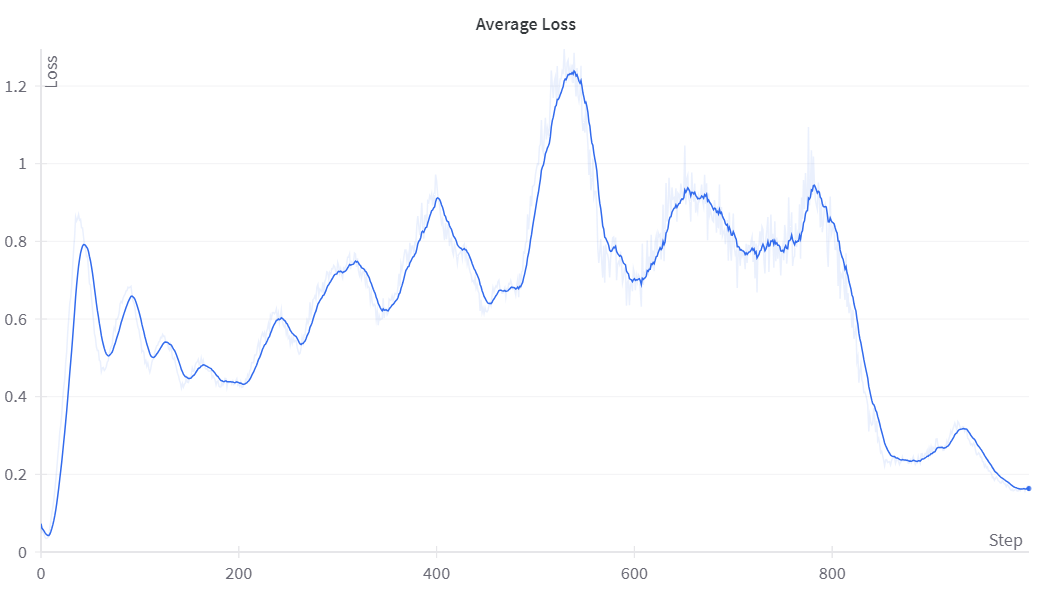
\includegraphics[width=\textwidth]{fig/new/DQNperdida.png}
        \caption{Pérdida promedio del modelo DQN. La línea tenue en el fondo representa la señal completa, y la línea oscura dicha señal filtrada para rescatar su tendencia.}
        \label{fig:LosspromDQN}
    \end{subfigure}
    \caption{Proceso de entrenamiento recompensa-pérdida de la implementación DQN con entorno PAMH.}
    \label{fig:PromDQN}
\end{figure}

\begin{figure}[hh]
	\centering
	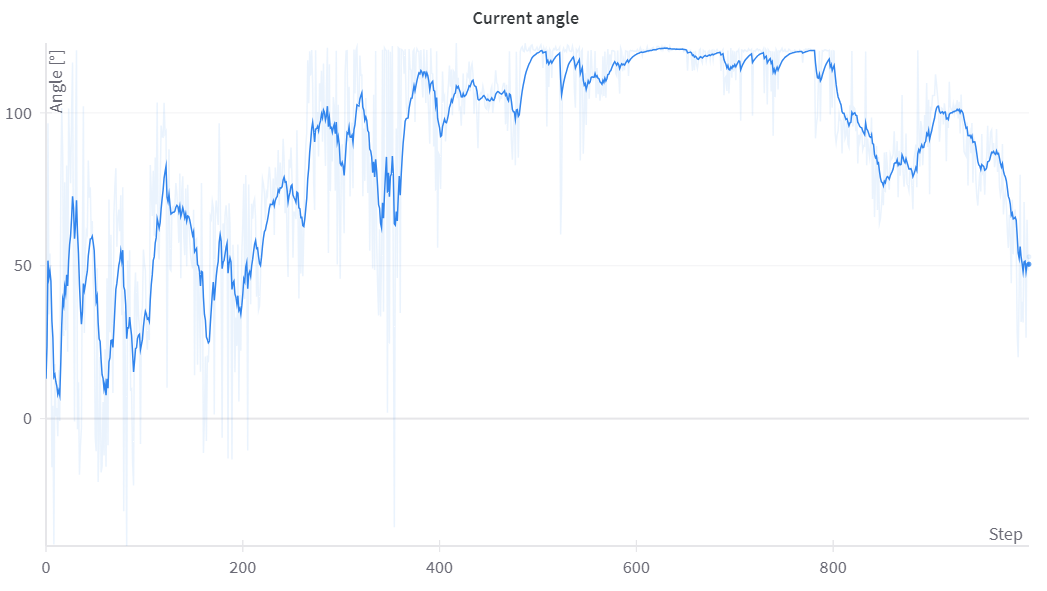
\includegraphics[scale=0.43]{fig/new/DQNentrenadosang.png}
	\caption{Últimos ángulos muestreados de los episodios del entrenamiento DQN con PAMH. La línea tenue en el fondo representa la señal completa, y la línea oscura dicha señal filtrada para rescatar su tendencia.}
	\label{fig:AnglepromDQN}
\end{figure}

Además, los comportamientos descritos pueden estar directamente relacionados el factor ``discretización'', pues el modelo parece aprender una buena táctica en los puntos indicados, pero pierde el rumbo o se queda sin posibilidades para alcanzar el objetivo, por lo que puede estar relacionado con una decisión de no aumentar o dividir el PWM y pasarse de lejos el $\theta_{objetivo}$.


\subsection{Modelo PPO}

Luego de aplicar el algoritmo base PPO con los cambios resaltados en el capítulo \ref{ch:ControlPAMH}, el proceso de entrenamiento demostró resultados prometedores desde la perspectiva del RL, ilustrados en la figura \ref{fig:Rewsprom}, donde se muestra el efecto del cambio del hiperparámetro varianza $\sigma^2$ en la curva, pues está directamente relacionada con el rango posible de valores alreatorios al que el agente se ve expuesto en la etapa de exploración. La curva rosa se expone a menos posibilidades de acción, pero la eficiencia del modelo permite que de igual forma converga a una recompensa positiva de aproximadamente $0.2$, sin embargo, puede tratarse de un caso de éxito con poca experiencia, donde un  pequeño desajuste podría desequilibrar por completo al modelo. 

La curva verde con el hiperparámetro fijo en $\sigma^2=0.01$, muestra una convergencia lenta en comparación, apenas llegando a $-0.175$ aproximadamente, pues el ``ruido'' experimentado agrega complejidad a la búsqueda del $\theta_{objetivo}=45^o$, requiriendo mayor tiempo de entrenamiento. Es posible proyectar un escenario donde a pesar del aumento de la recompensa, el agente nunca pueda llegar al valor deseado $\theta_{objetivo}$ o caso contrario, alcanzar el objetivo con el modelo de mayor experiencia frente a desequilibrios.

La curva morada muestra una convergencia satisfactoria a una recompensa superior al $0.2$ de la curva rosa, pero contando con una experiencia o política más completa de las técnicas para llegar al objetivo, esto gracias a la variación o barrido de valores de $\sigma^2$, de modo que el ruido produce exploracíon suficiente para luego dar paso a la explotación de lo aprendido. Por lo tanto, representa el modelo mejor preparado.

También es posible observar en la figura \ref{fig:Angleprom} el valor final del ángulo por episodio, donde las tres curvas tienden al $\theta_{objetivo}=45^o$, pero la curva rosa no exploró los ángulos lejanos y la curva verde requiere mayor estabilidad hacia el objetivo; los tres casos son proyecciones equivalentes a su recompensa promedio.


\begin{figure}[hh]
	\centering
	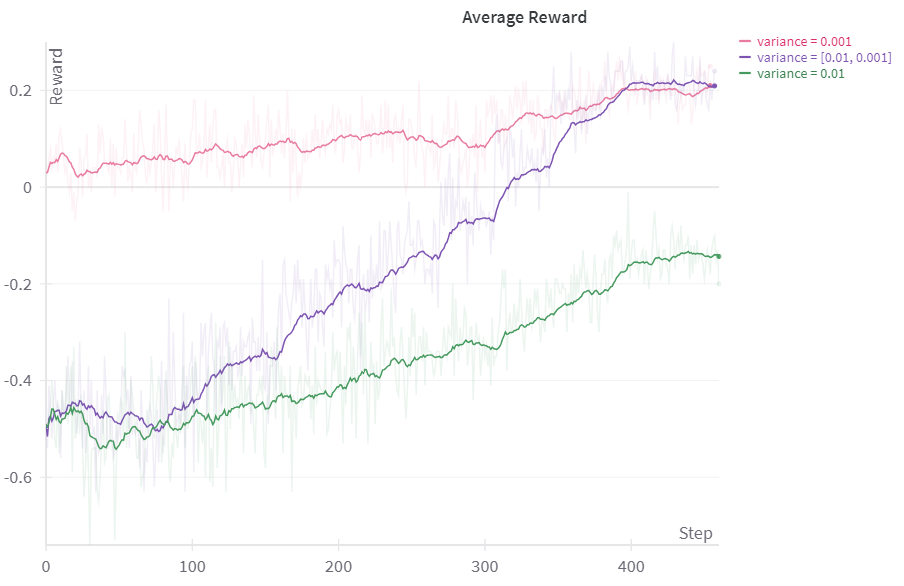
\includegraphics[scale=0.5]{fig/new/PPOentrenados.png}
	\caption{Recompensa promedio de los entrenamientos con diferentes valores de varianza $\sigma^2$. La curva rosa contempla $\sigma^2=0.001$, la curva verde contempla $\sigma^2=0.01$ y la curva morada contempla el barrido en el rango de $\sigma^2=[0.01, \,\, 0.001]$. Las líneas tenues en el fondo representan la señal completa, y las líneas oscuras dichas señales filtradas para rescatar sus tendencias.}
	\label{fig:Rewsprom}
\end{figure}

\begin{figure}[hh]
	\centering
	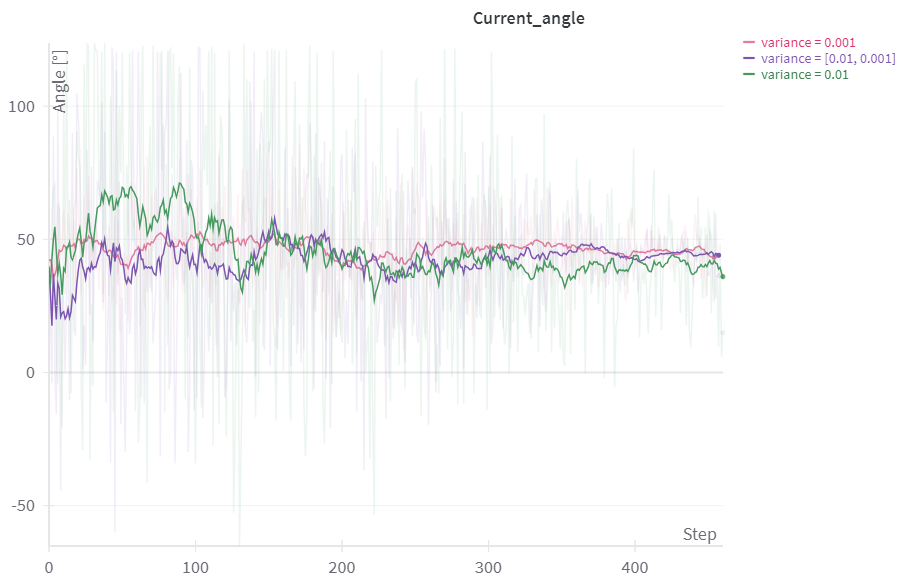
\includegraphics[scale=0.5]{fig/new/PPOentrenadosang.png}
	\caption{Últimos ángulos muestreados de los episodios en el entrenamiento. La curva rosa contempla $\sigma^2=0.001$, la curva verde contempla $\sigma^2=0.01$ y la curva morada contempla el barrido en el rango de $\sigma^2=[0.01, \,\, 0.001]$. Las líneas tenues en el fondo representan la señal completa, y las líneas oscuras dichas señales filtradas para rescatar sus tendencias.}
	\label{fig:Angleprom}
\end{figure}


\section{Evaluación del desempeño de los métodos RL}

La prueba final de evaluación requiere observar el efecto directo de la RNA entrenada frente al entorno sin perturbaciones o etapas de entrenamiento dictadas, únicamente la respuesta directa de la RNA.

Como se observó en la figura \ref{fig:RewspromDQN}, el método DQN no llega de manera certera al ángulo objetivo, por lo cual los parámetros de control no son medibles, sin embargo, muestra intentos de aprendizaje con el aumento de recompensa en algunos periodos y al alcanzar el objetivo, pero de forma casi inmediata se pierte el avance, por lo que su comportamiento es de un sistema no amortiguado como se muestra en la figura \ref{fig:DQNfinal}, donde se agrega la señal PWM resultante que el agente aplica para el control. El algoritmo no logra encontrar una política para determinar las acciones discretas que conducen al comportamiento objetivo.
 
\begin{figure}[hh]
	\centering
	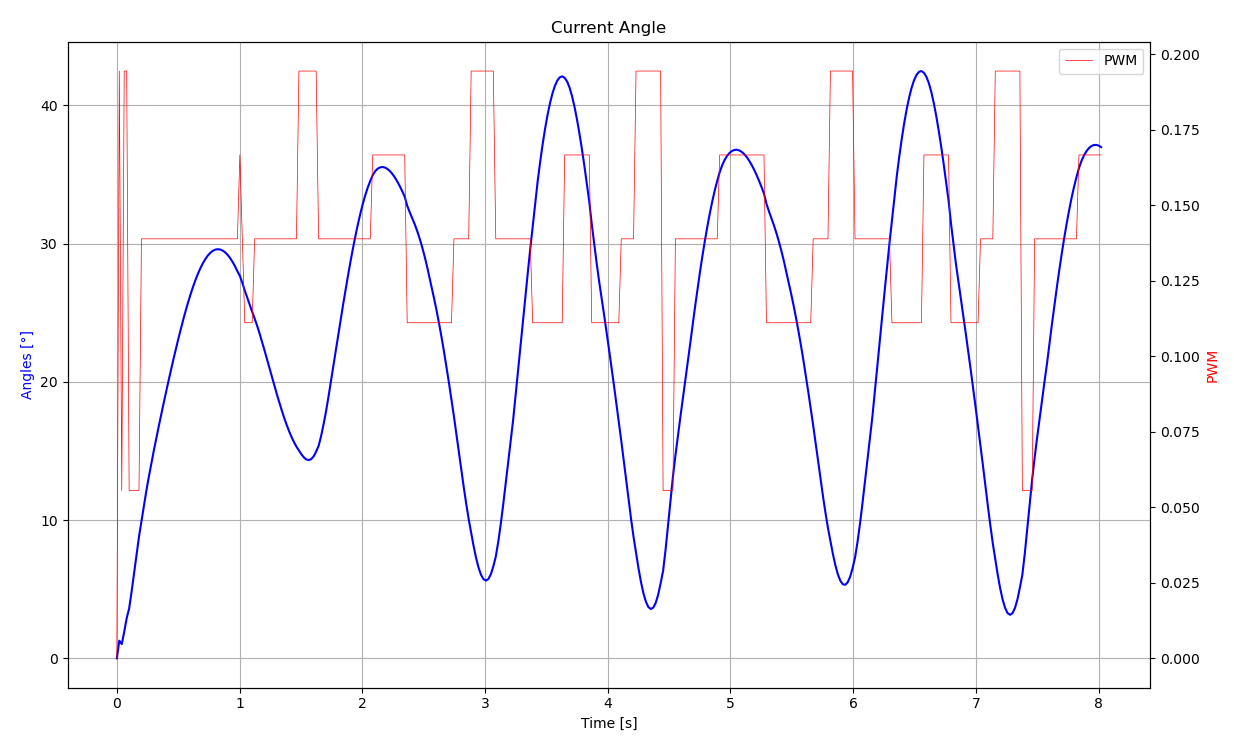
\includegraphics[scale=0.4]{fig/new/DQNprueba.png}
	\caption{Curva de respuesta del modelo DQN ángulo respecto al tiempo.}
	\label{fig:DQNfinal}
\end{figure}


En cuanto al modelo entrenado con PPO, se tiene la curva de la figura \ref{fig:PPOfinal} donde se observan, a pesar del comportamiento durante el entrenamiento, el efecto de subamortiguado, pues la oscilación hacia el valor final es alta y requiere más de $14\, s$ para alcanzar un estado de reposo, que también se trata de un valor incorrecto, aproximado a $29^o$. Además, los datos experimentales medidos fueron: tiempo de subida $t_r = 0.2603. \, s$, tiempo de estabilización $t_s = 15.78\, s$ y un sobreimpulso de $M = 75.66\%$.

Si bien estos valores son deficientes desde la perspectiva del control automático, se anota que estas métricas no han sido consideradas aun dentro de la función de recompensa, que en este caso solo incluye términos para el error angular y la velocidad terminal del péndulo. Las curvas de entrenamiento muestran que, incluso con la perturbación con el ruido del proceso de entrenamiento, el ángulo sí converge a los $45^o$, pero no se ha logrado encontrar la causa de por qué en la puesta a prueba del modelo aislado lleva a otro ángulo.


\begin{figure}[hh]
	\centering
	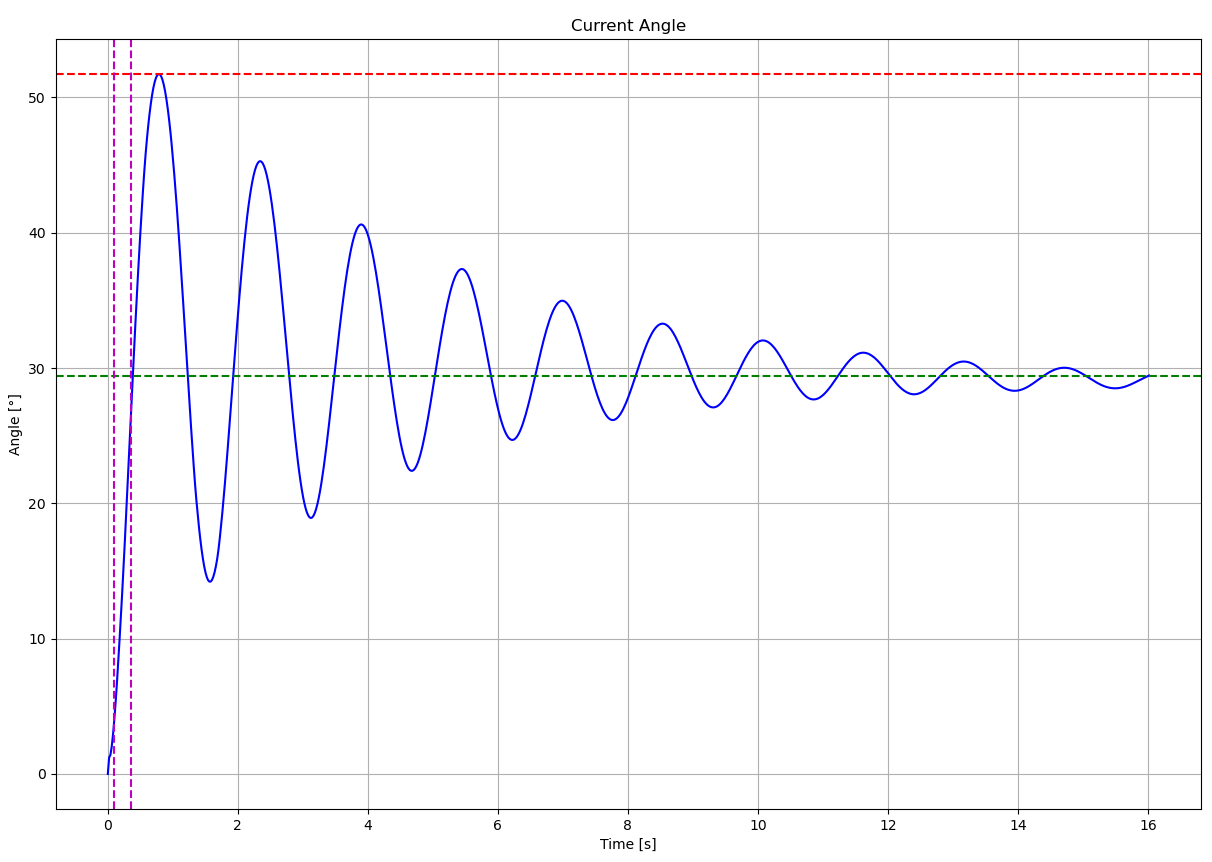
\includegraphics[scale=0.4]{fig/new/PPOprueba.png}
	\caption{Curva de respuesta del modelo PPO ángulo respecto al tiempo.}
	\label{fig:PPOfinal}
\end{figure}


